\chapter{Introduction}
\label{ch:intro}

\section{Motivation}
\label{sec:motivation}
Despite advances in solar technology and reduced costs, high upfront installation costs remain a barrier for residential users in developing regions. Pay-as-you-go financing models have expanded solar access but introduce challenges for providers: payment compliance monitoring, system performance tracking, tampering detection, and remote management.

The Solar Energy Monitoring and Control System addresses these challenges through automated monitoring, consumption tracking, payment compliance, and security features, reducing operational overhead while expanding solar accessibility.

\section{Purpose of the System}
\label{sec:purpose}
The Solar Energy Monitoring and Control System is designed to monitor, analyze, and manage solar installations. Primary goals include: (1) real-time energy production and consumption monitoring, (2) automated energy summaries (daily, weekly, monthly), (3) financial management including payment plans and compliance, (4) analytics for data-driven decisions, and (5) security through tampering detection and authentication mechanisms.

\section{Key Features}
\label{sec:keyfeatures}

\subsection{Energy Monitoring}
\label{subsec:energymonitoring}

The Energy Monitoring module provides: real-time tracking of energy production and consumption via WebSocket, batch processing of historical energy readings, automated daily/weekly/monthly summaries with statistics, dashboard visualizations with chart data, and energy analytics for performance insights.



\subsection{Payment Compliance}
\label{subsec:paymentcompliance}

The Payment Compliance module manages installment-based solar financing: flexible payment plan configuration with multiple frequencies (weekly, bi-weekly, monthly, quarterly, semi-annually, annually), automated payment status tracking and updates, payment reminder system with configurable grace periods, comprehensive payment history and dashboard analytics, receipt generation, overdue payment identification, and manual payment recording for administrative use.



\subsection{Security and Tampering Detection}
\label{subsec:security}

The Security module includes: tamper event detection and logging (physical, voltage, connection, location types), severity-based classification and filtering, alert configuration and notification system, real-time tamper event reporting via WebSocket, resolution tracking and acknowledgment workflows, and security audit logging for compliance.



\subsection{User Management}
\label{subsec:usermanagement}

The User Management module provides: role-based access control (Admin/Customer), secure authentication with JWT tokens, email-based account activation and password reset, profile management and update capabilities, and user activity tracking.



\subsection{Service Control}
\label{subsec:servicecontrol}

The Service Control module enables remote management of solar installations: automated service activation/deactivation based on payment compliance, manual override controls for administrators, scheduled disconnections, reconnection workflows, and operational logging for compliance and troubleshooting.

\section{System Architecture Overview}
\label{sec:architecture}

The system employs a modular monolithic architecture with six key modules: Energy Monitoring, Payment Compliance, Security and Tampering Detection, System Monitoring, User Management, and Frontend Application. This approach ensures maintainability and clear separation of concerns \cite{newman2021building}.

\begin{figure}[h]
    \centering
    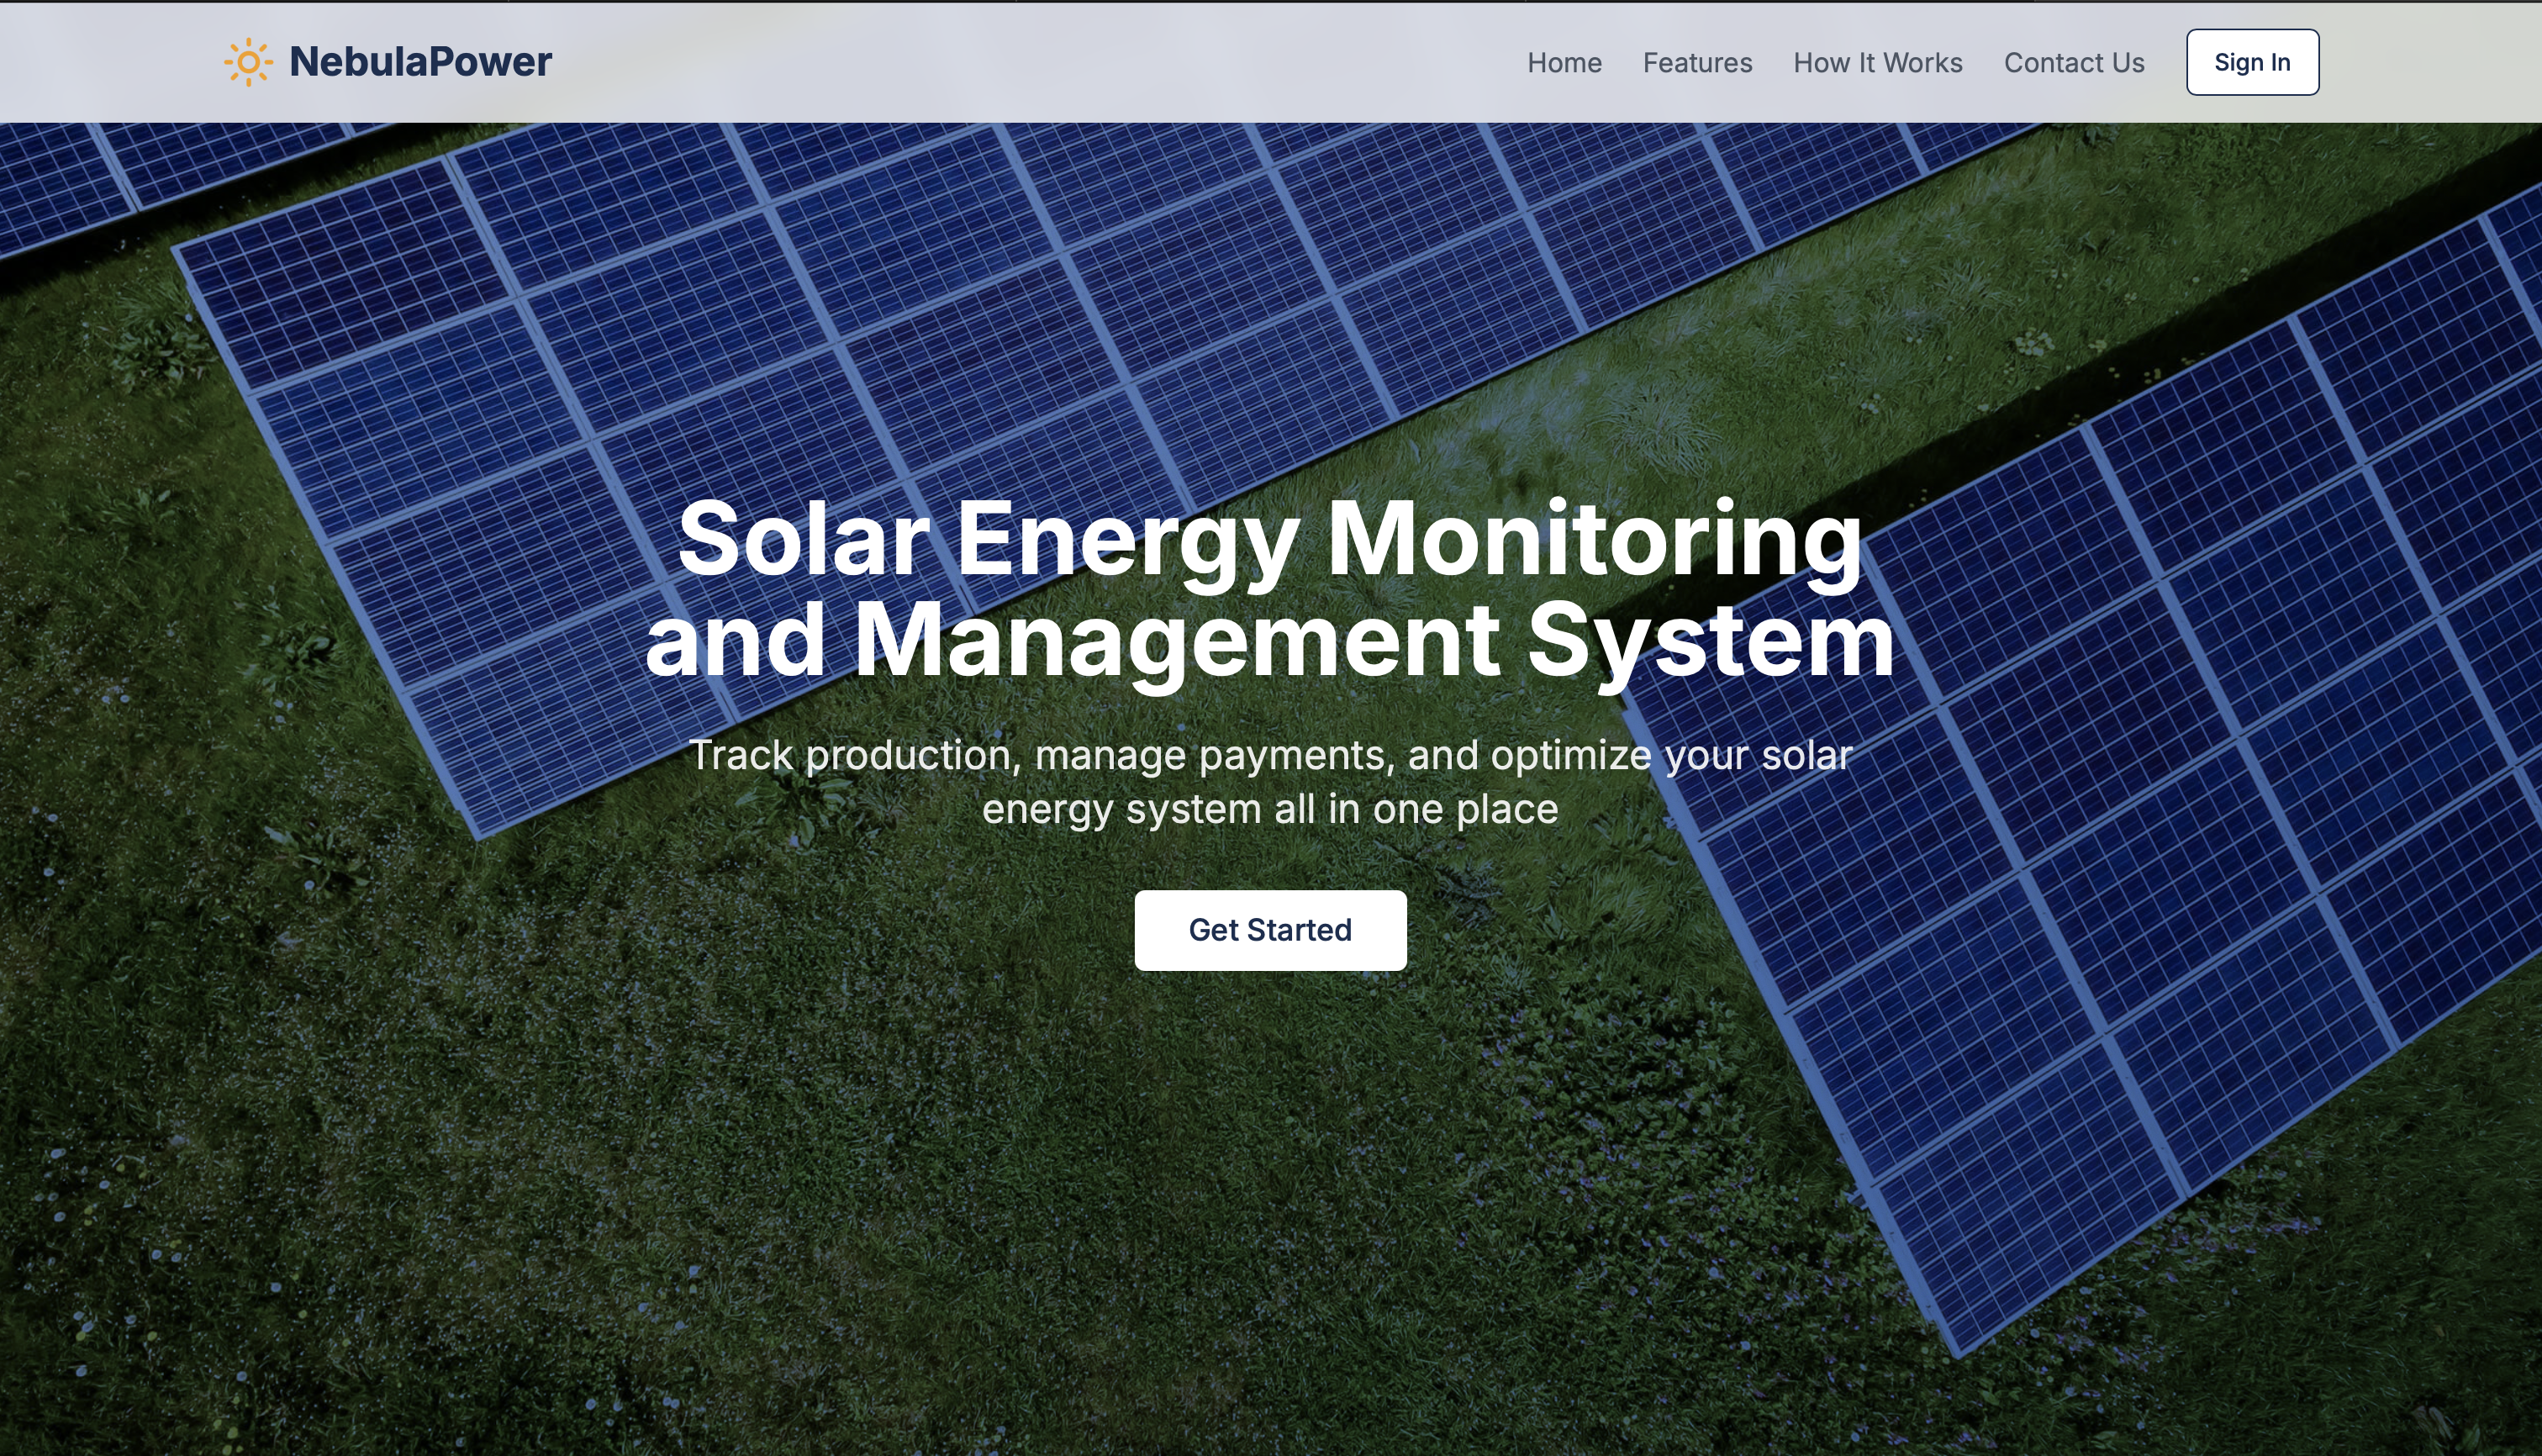
\includegraphics[width=1.1\textwidth]{images_2/landing_page.png}
    \caption{Solar Energy Monitoring and Control System platform landing page}
    \label{fig:architecture}
\end{figure}

\section{Thesis Structure}
\label{sec:structure}

This thesis is organized into the following chapters:

\begin{itemize}
    \item \textbf{Chapter 1: Introduction} - Provides the context, motivation, and high-level overview of the Solar Energy Monitoring and Control System platform.
    
    \item \textbf{Chapter 2: User Documentation} - Detailed documentation for end-users, including installation guides, user interfaces, and operational procedures.
    
    \item \textbf{Chapter 3: Developer Documentation} - Technical documentation covering system architecture, implementation details, APIs, and development guidelines.
\end{itemize}

Each chapter is designed to provide comprehensive information for its target audience, whether they are end-users interacting with the system or developers extending or maintaining the platform.
